\documentclass[12pt,twoside,a4paper]{scrartcl}

\usepackage{prakstyling}
\usepackage[paper=a4paper,left=20mm,right=20mm,top=20mm,bottom=20mm]{geometry}
\usepackage{wrapfig}
\usepackage{amsmath}
%Für Literaturverzeichnis

\usepackage{biblatex}
\addbibresource{Bibliography.bib}



%%%%%%%%%%%%%%%%%%%%%%%%%%%%%%% Autoreninfo %%%%%%%%%%%%%%%%%%%%%%%%%%%%%%%%%%%%%%%%%%%%%%%%%%
\author{Philipp Rosendahl Mat.-Nr: 378029\thanks{philipp.rosendahl@rwth-aachen.de}
		\and Lennart Wilde, Mat.-Nr: 381588\thanks{lennart.wilde@rwth-aachen.de}}

\pSetShortAuthor{378029 \& 381588}
%%%%%%%%%%%%%%%%%%%%%%%%%%%%%%%%%%%%%%%%%%%%%%%%%%%%%%%%%%%%%%%%%%%%%%%%%%%%%%%%%%%%%%%%%%%%%

%%%%%%%%%%%%%%%%%%%%%%%%%%%%%%%%%%%%%%%% TITEL %%%%%%%%%%%%%%%%%%%%%%%%%%%%%%%%%%%%%%%%%%%%%%
\pSetTitlePrefix{Versuch}
\pSetTitleNumber[PET]
\pSetLongSubject{Physikalisches Fortgeschrittenenpraktikum - Gruppe 59} \pSetShortSubject{Gruppe 59}
%%%%%%%%%%%%%%%%%%%%%%%%%%%%%%%%%%%%%%%%%%%%%%%%%%%%%%%%%%%%%%%%%%%%%%%%%%%%%%%%%%%%%%%%%%%%%

\setlength{\parindent}{0pt}
\pagenumbering{roman}

\raggedbottom

\renewcommand{\tablename}{Tab.}
\renewcommand{\figurename}{Fig.}
\setlength{\abovecaptionskip}{1ex}
\setlength{\belowcaptionskip}{1ex}
\setlength{\floatsep}{1ex}
\setlength{\textfloatsep}{1ex}

\begin{document}

\maketitle
\newpage

\tableofcontents
\newpage

\pagenumbering{arabic}

\section{Einleitung}
	
	Die PET ist ein wichtiges Bildgebendes Verfahren in der modernen Medizin um auch kleine Tumore im menschlichen Körper ausfindig zu machen. Daher ist die Entwicklung leistungsfähiger Detektoren ein wichtiger Aspekt moderner Forschung. \\

	Das zugrunde liegende Prinzip basiert auf der besonders hohen Biologischen Aktivität von Tumorgewebe. Wir einem Patienten nun ein mit einem Radioaktiven Isotop markierter Zucker (sog. Tracer) verabreicht, sammelt sich dieser in dem Tumor an. Wenn dieser nun zerfällt emittiert er Positronen die sich mit den Elektronen im umliegenden Gewebe auslöchen und zwei Gamma Photonen in entgegengestezte Richtung aussenden. Diese sollen durch die Detektoren aufgefangen und ausgewertet werden um Informationen über Flugzeit und Energie der Strahlung zu erhalten. Für die Konstruktion dieser Detektoren gibt es mehrere Ansätze, allerdings wurde in diesem Experiment ein Silicon-Photomultiplier (SiPM) zusammen mit einem LYSO Szintillator verwendet.\\

	Ein auftreffendes Gamma-Photon regt den Szintillierenden Kristall nun an optische Photonen auszusenden, die auf den SiPM treffen. Dort werden sie in ein elektrisches Signal umgewandelt, welches durch einen ASIC ausgelesen und verarbeitet werden kann, um aus der Anzahl der Photonen die Energie des detektierten Photons sowie die Flugzeit udn Position zu rekonstruieren. In einem mdeizinischen PET-Scanner kann mit diesen Informationen nun die lage der Tumoren im Patienten errechnet werden. In diesem Versuch ist allerdings eher die Vermessung des verwendeten Detektors im Fokus, weswegen nur zwei sich gegenüberstehende Detektoren verwendet werden.

	\newpage

\section{Versuchsaufbau}
	
	Der Aufbau besteht aus verschiedenen Teilen:
	\begin{itemize}
		\item Dunkelbox mit 
		\begin{itemize}
			\item 2 $\gamma$-Detektoren
			\item Backbone
			\item Aluminiumgstell mit Schrittmotoren für Probenhalter
			\item Probenhalter für Radioaktive Probe
			\item 
		\end{itemize}
		\item Netzteile für Detektoren und Backbone
		\item Data Aquisition and Processing Server (DAPS)
		\item Kühlung
		\item Steuerungsrechner mit Benutzerinterface
	\end{itemize}

	\begin{figure*}[H]
	
		
		\begin{minipage}{0.25\textwidth}

					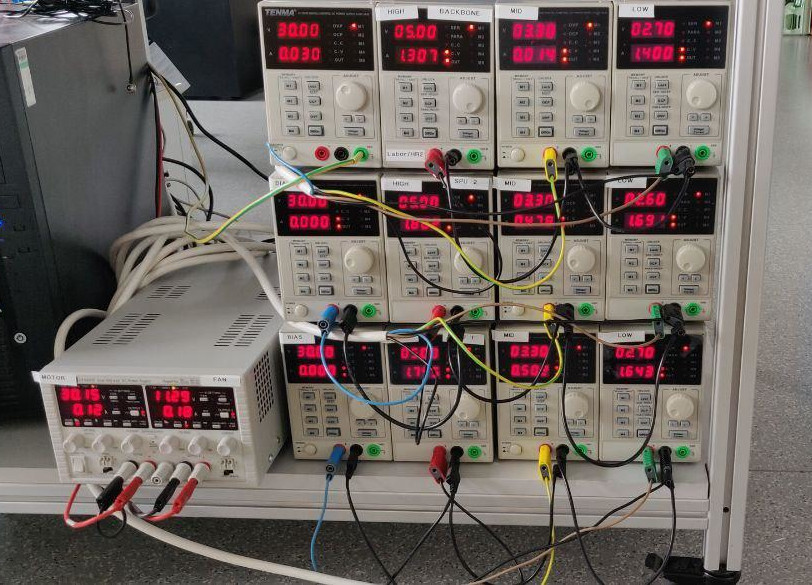
\includegraphics[width = 0.2 \textwidth]{Bilder/Netzteile.jpeg}
					\label{Aufbau::Netzteile}
					\caption{Netzteile mit verschiedenen Spannungen}

		\end{minipage}
		\begin{minipage}{0.25\textwidth}

					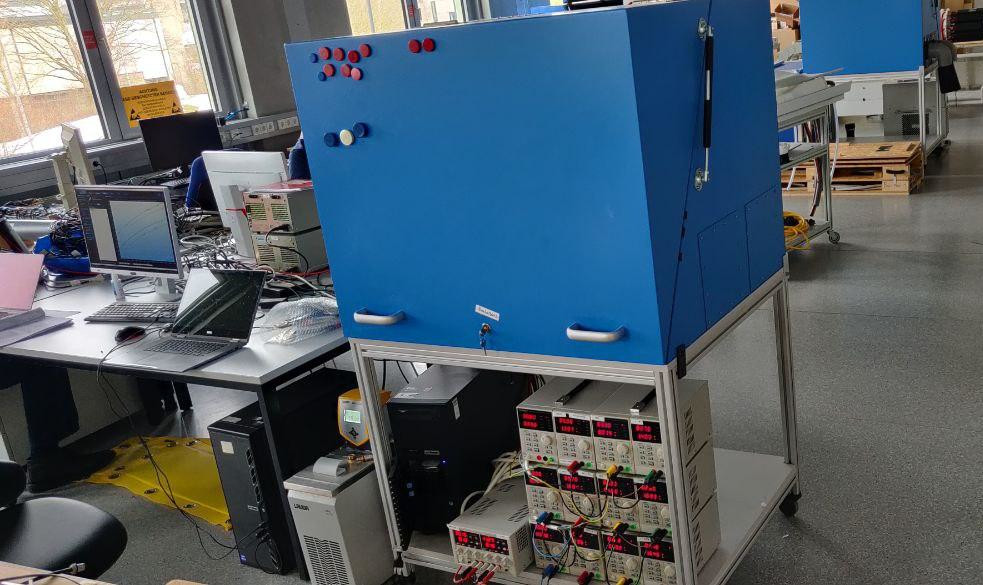
\includegraphics[width = 0.2 \textwidth]{Bilder/Kammer.jpeg}
					\label{Aufbau::Kammer}
					\caption{Geöffnete Dunkelkammer}

		\end{minipage}
		\begin{minipage}{0.25\textwidth}
		
					\includegraphics[width = 0.2 \textwidth]{Bilder/Kühlung.jpeg}
					\label{Aufbau::Kühlung}
					\caption{Wasserkühlung}
		\end{minipage}

	\end{figure*}


	Um den Aufbau einzuschalten, muss zuerst die Kühlung gestartet werden. Danach werden die LOW, MID und HIGH Spannungen des Backbone in dieser Reihenfolge eingeschaltet. Daraufhin bootet dieser, wobei der vollständige Start durch einen Sprung in der Stromaufnahme der HIGH-Versorgungsspannung festgestellt werden kann. Nachdem der Backbone gestartet ist, können die 2 Detektoren (SPUs) eingeschaltet werden, indem wie schon bei dem Backbone zuerst die Versorgungsspannungen in der Oben angegebenen Reihenfolge sowie die BIAS-Spannung eingeschaltet werden. Auch hier ist die Betriebsbereitschaft durch einen Sprung in der Stromaufnahme auf ungefär 1.6 A erkennbar. Nun kann der Steuerungsrechner mit dem Aufbau verbunden werden. Dazu startet man die "Hyperion" Software und führt dort das zu dem Versuch gehörenden Startskript aus. Daraufhin wird eine Verbindung hergestellt, die Detektoren initialisiert und mit dem Backbone synchronisiert. Aufgrund von sporadisch auftretenden Verbindungsproblemen zwischen Backbone und den SPUs kann dieser Schritt fehlschlagen, worauf dann die Spannungen un der umgekehrten Reihenfolge abgeschaltet und der Aufbau neu gestartet werden muss.
	Ist erfolgreich eine Verbindung zwischen allen Komponenten hergestellt, sollte spätenstens nun die Dunkelkammer geschlossen werden, da im nächsten Schritt die Bias-Spannungen an die SiPMs angeschlossen werden. Wären diese nun nicht im dunklen würden sie konstant ausgelöst, was Messungen unmöglich macht und sie außerdem beschädigen kann. Ist die Kammer also geschlossen, kann mit dem Skript "Continue\_Start" der Aufbau in einen Messbereiten Zustand versetzt werden.

	\section{Dark Count Map}

		\subsection{Aufbau und Durchführung}

			Aufgrund des thermischen Rauschens der Dioden, sowie Herstellungsprzessen und -ungenauigkeiten haben diese eine sog. "Dunkelzählrate", d.h. eine Signalausgabe bei nicht vorhandener Stimulation. Um nun einzelne Dioden mit besonders hoher Rate zu erkennen und abzuschalten, wird vor der ersten Messung eine "Dark Count Map" der SiPMs ohne eine Probe erstellt. Mithilfe dieser kann man nun ermitteln welche SPADs abgeschaltet werden sollten, um eine Reduzierung der Dunkelzählrate ohne eine zu hohe Reduktion der anderen Genauigkeiten zu errreichen.\\
			Zur Durchführung der Messung wird der Aufbau wie oben beschrieben eingeschaltet und das Skript zum durchführen der Messung gestartet. Diese dauert einige Minuten, und nach Abschluss werden die Daten auf dem DPAS gespeichert und müssen von dort auf den Rechner übertragen werden.

		\subsection{Auswertung}

			Die aus der Messung erhaltenen Daten lagen als eine Datei mit Tab seperierten Werten (TSV) vor (siehe Rochdatenverzeichnis). Um eine einfache Übersicht über die Sensoren zu erhalten wurde die Datei nun meit einem Python Skript eingelesen und die enhalten Zählraten in einer 2D-Grafik angezeigt:

			\begin{figure*}[H]
				\begin{minipage}{0.49 \textwidth}
					\includegraphics[width = \textwidth]{Plots/DCM_1.eps}
					\caption{Dark Count Map von SPU 1}
				\end{minipage}
				\begin{minipage}{0.49 \textwidth}
					\includegraphics[width = \textwidth]{Plots/DCM_2.eps}
					\caption{Dark Count Map von SPU 2}
				\end{minipage}
			\end{figure*} 

			Außerdem wurde die Gesamtzählrate in Abhängigkeit von den abgeschalteten SPADs mit besonders hoher Rate ermittelt:

			\begin{figure*}[H]
				\includegraphics[width = 0.5 \textwidth]{Plots/DCR.eps}
				\caption{Dunkelzählrate der SPUs}
			\end{figure*}

		\subsection{Fazit}

		Man sieht das N SPADs für einen Großteil des Rauschens sorgen der durch die Abschaltung dieser eliminiert werden kann. Für die weiteren Messungen ist sies leider nicht sonderlich relevant, da für die Sensoren vorkonfigurierte Prarameter verwendet wurden, in die wir leider keine Einsicht hatten.

	\section{Rauschmessung}
	

	\section{Detektoreffizienz und Count Rate}

		\subsection{Aufbau und Durchführung}

		\subsection{Auswertung}

		\subsection{Fazit}

	\section{Energiemessung}

\end{document}
